\section{爆炸反射面}
脉冲波震源、检波器(有时像个拾音器)和多记录道波形显示系统是反射地震勘探的基
本设备。测线沿地表布置,对海上勘探而言,测线可以是指勘探船航道,在这种情形下,接
收装置称作水听器。大约每25米震源激发一次,并在附近记录回声。由于穿透地层的池震波
波长比勘探船还长,震源和水听器几乎没有什么方向调谐能力,因此,回声可同时从几个方
向到达。解释这些观测结果,是地球物理学家和地质学家的共同任务。地球物理学家承担定
量的、物理的和统计方面的任务,他们的主要目标(因而也是主要指导写作本书的目标)就
是根据这些回声作出有关地层内部的良好图像。

\subsection{有力的类比}

图\ref{fig:xrf/expref}所示是两神波动传播情
形,第一种情况是实际的野外回声测深方法,第二种情况是一个想象的观
测记录情况------地层内的反射面突然
同时爆炸激发,从假设的爆炸震源产 生的波向上传播至地面,为假设的一
组检波器所接收。

\begin{figure}[H]
\centering
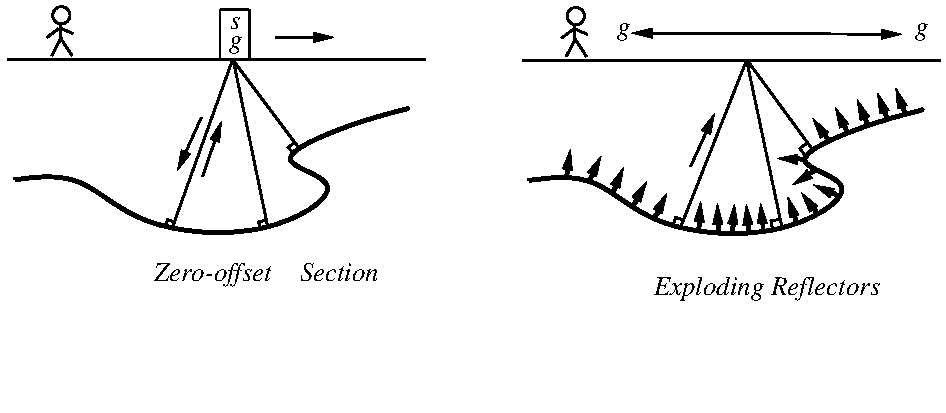
\includegraphics[width=0.95\textwidth]{xrf/expref}
\caption[爆炸反射面]{沿地表面所有位置移动的自激自收方式回声采集(左图),“爆炸反射面”想象模型(右图)}
\label{fig:xrf/expref}
\end{figure}
在图中要注意,实际野外记录情
形下的射线路程看起来同想象的爆炸 反射面情形下的那些射线路程是一样
的,把观测的与假设的这两种波场想像成确实是相同的波场,这在概念上有很大的好处。如果
它们相同,那么实际完成的成千炮记录就可忽略不计,从而可把注意力只集中于一个假设的记
录上。在实际的与想像的这两种情形 之间,有一种明显的差异,那就是:在实际野外观测系统中,
波必须首先 向下传播,然后沿同一路程向上返回
地表,而在假设的观测记录中,波只 向上传播;前者是双程射线路程,后
者是单程射线路程。野外实际观测记 录的旅朽时间应除以2;在实际工作
中,分析野外观测记录资料(双程时间)时都假设波速等于其真值的一半。

\subsection{惠更斯二次点源}
海面波浪具有可与地震勘探采用的波长相比的波长(15米至500米),不同之处就是海浪移动缓慢,容易观察。假设想
像有一很长的平行于海滩的码头防波堤,该堤有一很狭小的入口,恰可容许船只通过。这种
情形如图\ref{fig:xrf/storm}所示。来自开阔的公海而入射在防波堤上的。平面波将形成一个通过该堤空隙
的波。能观察到的一件事实就是:波阵面在码头内部变成为一个以该空隙为圆心的半圆弧。
波浪的这种波束与经过窗户射入的光线之间的差别只在于波长与孔穴大小之比值不同而已。

\begin{figure}[H]
\centering
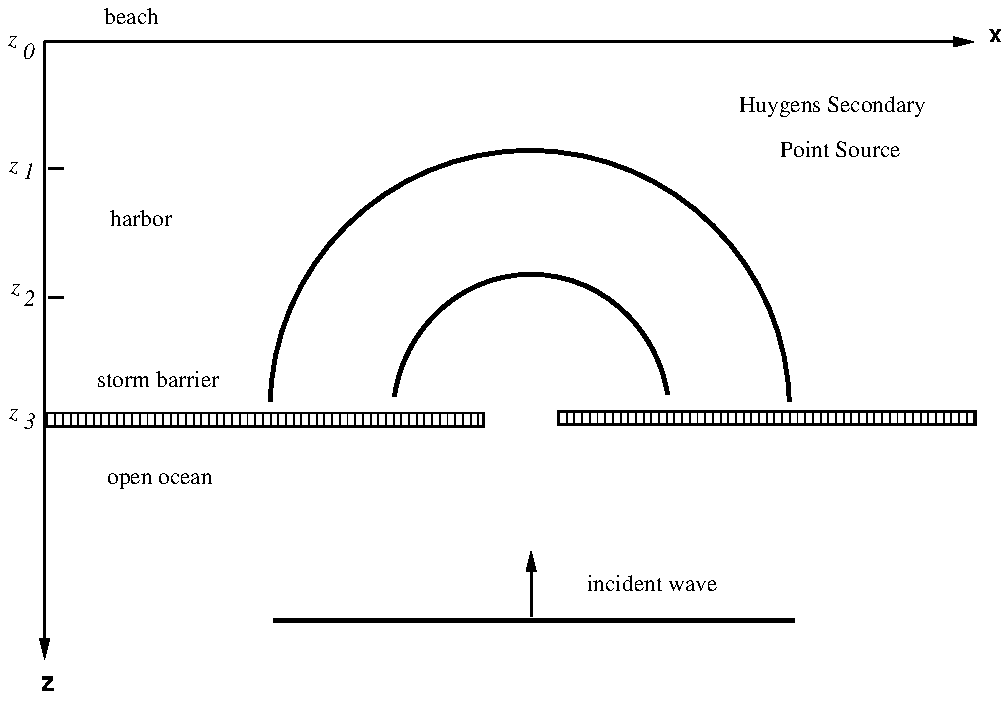
\includegraphics[width=0.6\textwidth]{xrf/storm}
\caption[惠更斯]{通过防波堤空隙的波具有半圆形波阵面(波长的长度可与空隙大小相比时)}
\label{fig:xrf/storm}
\end{figure}

线性性质是所有弱振幅波(不是指近岸处泡沫迸溅的碎浪)的一种性质,这意味着防波堤
有两个空隙就要形成两个半圆形波阵面,两圆相交处的波浪高度就等于两个高度的线性相加
结果。有趣的是考虑一下一个具有许多洞穴的防波堤,在洞穴非常多这种极限情形下,防波
堤消失了,剩下的只不过是一个紧挨着一个的空隙,许多半圆形波阵面形成的仅是入射平面
波。双曲线形的时距曲线亦复如此,图\ref{fig:xrf/storm2}所示是密度由左至右逐渐增大的许多双曲线,
所有非垂直角度方向上的波必然按某方式彼此叠加,使得除该平面波存在之外,其他一切均被压制抵消。

\begin{figure}[H]
\centering
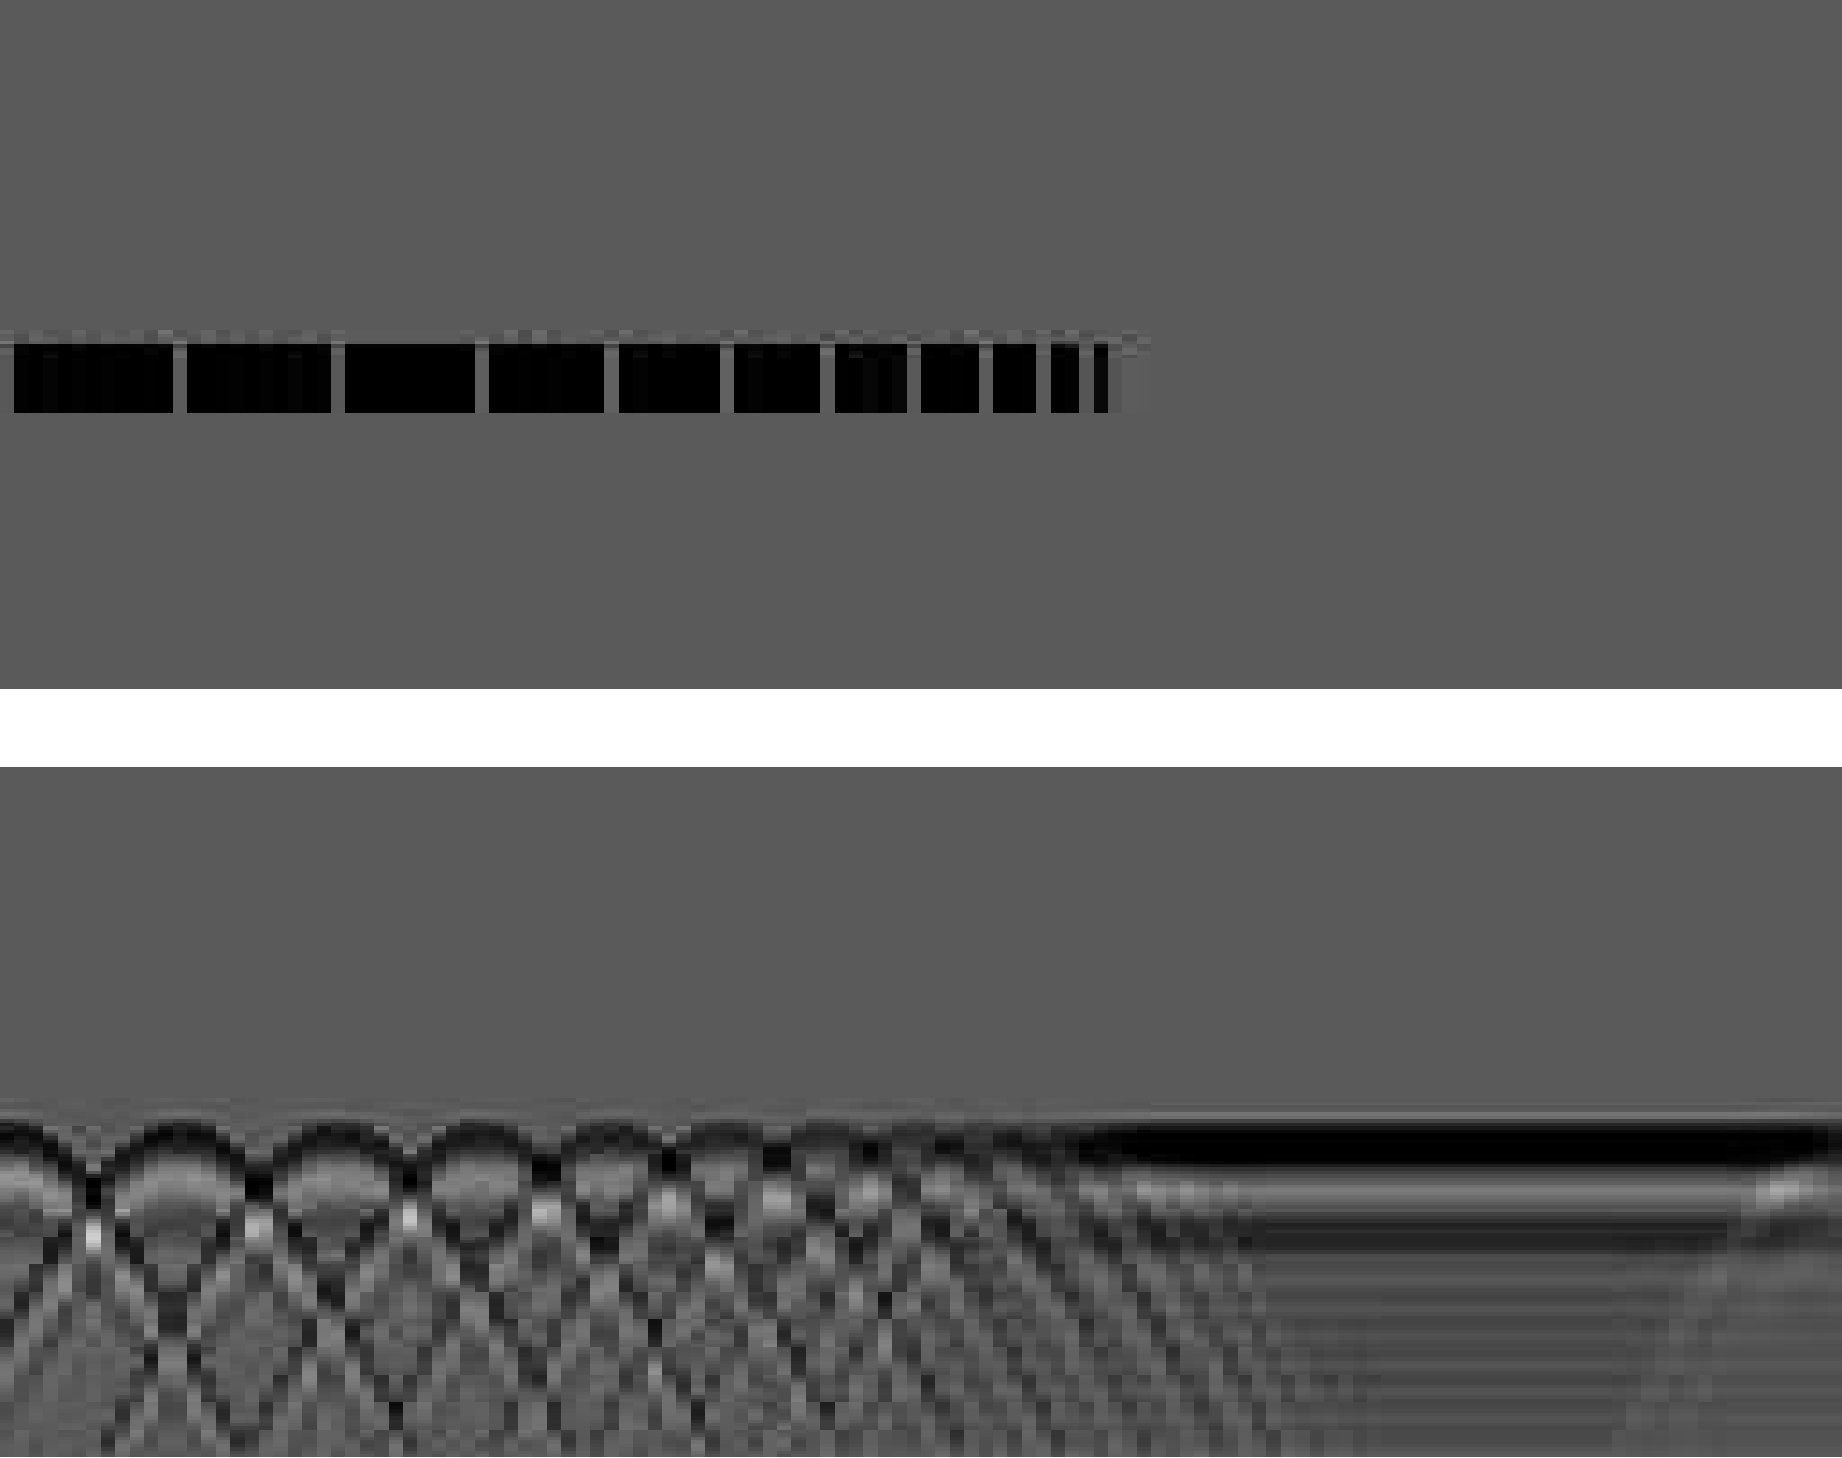
\includegraphics[width=0.95\textwidth]{xrf/storm2}
\caption[惠更斯]{具有许多洞穴的堤(顶部)及堤外所见到的$(x,t)$空间内的波(底部)}
\label{fig:xrf/storm2}
\end{figure}

设将直角坐标系统置于海面上,使海岸沿轴方向,而辅方向则可测度距海岸的距离。
为适合与反射地震学进行类比,假设人们活动只限于海岸(相当于反射地震中的地表面),
他们在那里进行波动观测------把波浪的高度作为坐标$x$与时间$t$的函数来加以观测记录。他们
根据这种数据可以作出关于在$(x,t)$平面内防波堤上存在有一个向外开口的空隙的推断。
图\ref{fig:xrf/dc}所示是波浪从海洋到达海岸的时间,最接近开口处之波浪最先到达,用什么数学
表达式来确定$(x,t)$平面内所见到約到达时间曲线形状呢?

\begin{figure}[H]
\centering
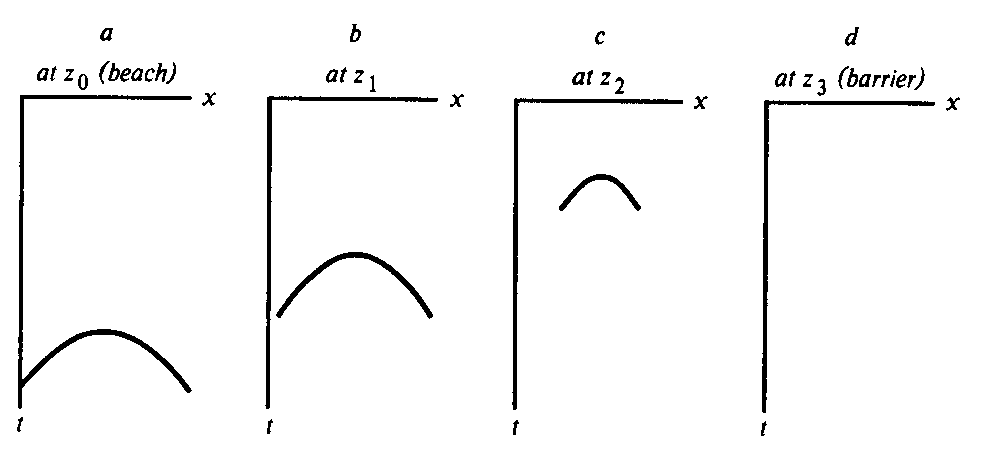
\includegraphics[width=0.95\textwidth]{xrf/dc}
\caption[dc]{左端的图表示在海岸上所见波浪之双曲线型时距曲线,右侧各图表示朝向海洋方向的距离子增大时,各个相继的到达时间曲线($x$轴业已压缩,不同于图\ref{fig:xrf/storm})(据Gonzalez)}
\label{fig:xrf/dc}
\end{figure}
波浪是一圈圈不断扩展着的圆。环绕点$(x_{3},z_{3})$以速度$v$不断扩张的圆其方程为:
\begin{equation}\label{eq:cir}
(x-x_{3})^{2}+(z-z_{3})^{2}=v^{2}t^{2}
\end{equation}
想像时间$t$为一常数时,即作一个快镜头拍摄时,则式\ref{eq:cir}就是那个圆的方程。设令$z$为
常数时,它就是在该$(x,t)$平面内的一个双曲线方程。若在三维体积内考
虑,式\ref{eq:cir}就是一个圆锥方程;各种不同$t$值时的横切面表现为各种不同大小的圆;各
种不同$z$值时的切片表示为各种不同的双曲线。图\ref{fig:xrf/dc}所示是四种双曲线,自左至右,第一
个双曲线是在海岸上$z_{0}=0$观测到的;第二个是在指向海洋方向的某个距离$z_{1}$上假想的一组
观测结果;第三个是在距海岸更远一些的距离$z_{2}$上假想的一组观测结果;第四个是在始终都
接近于防波堤的距离$z_{3}$上的一组观测结果,在该种情形下,双曲线业已蜕化为一个点。所有
这些双曲线均属于一个双曲线簇,每个双曲线均具有相同的渐近线。渐近线相应于在开口
空隙处转动将近90度角度的一种波,该波沿大约平行于海岸的方向移着,移动速度即波浪
速度$dx/dt$(为适合于对这种水波的类比,假定波浪的速度島一个与水深无关的常数)。

如果原始的入射波是个正脉冲,那么,惠更斯二次震源必然应由正极性与负极性二者组
成,才能使所有波动因相消干涉而彼此抵销,只有平面波存在。所以,惠更斯二次震源的波
形是有相移的。在下一节,将求出惠更斯二次震源的数学表达式。船工水手们熟悉的另一种
现象是:惠更斯半圆的最大振幅是位于直接指向海岸的方向上。由防波堤移动至海岸的波浪
系其振幅衰减至零,在光学中,这种随角度而出现的振幅减弱,称作倾斜因子(!obliquity!
 !factor!)。

\subsection{偏移定义}
!run!这个词,字典可以给出许多定义,它们彼此有关而又彼此有别。在地球物理勘探
中,!migration!(偏移)这个词同样也是大概有四种彼此有关而又彼此有区别的意思,最简
单的意思是像!move!(移动)这个词的意义。当位于$(x,z)$平面内某个位置上的物体在随后
时刻$t$时又位于另一个不同的位置上,于是我们就说它移动了。类似地,当位于地球物理观测
$(x,t)$空间内某个位置上的波至(往往也称作同相轴),又可在较大的深度$z$上出现在不同
位置上,于是我们就说它偏移了。

为更清楚看出这点,试想像图\ref{fig:xrf/dc}是取自一部影片的四个镜头画面。在影片放映时,
深度$z$就开始从海岸位置的深度(地表面)一直改变到防波堤位置的深度。把这些镜头画面叠合在一起,则
如图\ref{fig:xrf/dcretard}(a)所示。电影中发生的现象主要是同相轴朝$t=0$方向向上偏移了。
要消除这种占主导地位的垂直转移的影响,使各双曲线的顶点都保持在相同位置上进行另一种形式的叠加。
从数学上说,这就是用所谓的延迟时间轴$t^{'}=t+z/v$来代替时间轴$t$,如图\ref{fig:xrf/dcretard}(b)所示。

\begin{figure}[H]
\centering
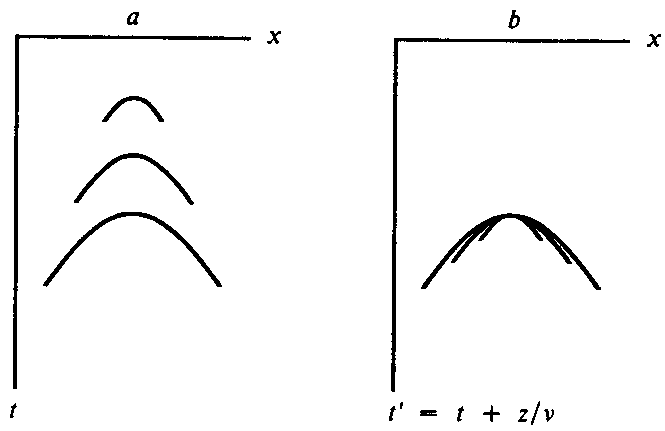
\includegraphics[width=0.95\textwidth]{xrf/dcretard}
\caption[dcretard]{(a)表示图\ref{fig:xrf/dc}中诸双曲线的叠合,(b)表示对叠合再配合以称作延迟$t^{'}=t+z/v$
的时移,使双曲线顶部彼此重叠(据Gonzalez)}
\label{fig:xrf/dcretard}
\end{figure}

第二种定义,也即更为准确的偏移定义是:在$(x,t^{'})$空间中的同相轴随深度$z$之改变而发生的移动。
在消除垂直时移之后,还有残余时间移动,那就主要是由某种波形变化引起的了。按照这种定义,双曲线
顶点或者水平地层是不偏移的。

图\ref{fig:xrf/dcretard}中的双曲线实际上是延伸至无限远的,但是图中每一个双曲线都在某个时间上
截断,这个时间等于$\sqrt{2}$乘该双曲线顶点的时间,所以图中所示双曲线仅是描述在与垂直方
向呈45度角的范围之内的射线。务必记住这一点:双曲线极小值时间与任何其它到达时间的比
值等于传播角度的余弦值。每个双曲线都是截止于45°出射角的射线。注意,图形上各双曲线
的端点可用一条直线连起来,还有,各双曲线端点上的斜率均相同,对于任何波阵面,波的传播角度在物理空间内为
$tan\theta =dx/dz$;对于任何地震同相轴,当你阵面以角度$\theta$与地面相交时,你就会发现,斜率$vdt/dx$
就等于$sin\theta$。所以,在物理空间$(x,z)$内沿一直线移动的能量就沿数据空间$(x,t)$内的一条直线而偏移。随$z$
之增大,沿所有角度传播的能量就一起聚集在一焦点上,这个焦点位于爆炸反射面,它就是防波堤内的开口空隙。这就是偏移
的第三种定义,即,偏移即是以某种方式将观测数据——作为$x$与$t$之函数的波浪高度——从海岸延展至防波堤的过程。第三种定义
并不过分强调移动本身,而是强调自起点至终点时的变换。

为更深入一步理解,只靠防波堤的例子是不行的,需要有更具普遍性的例子.防波堤的例子局限于仅在
某个特定深度$z$上形成惠更斯二次震源,但是为解释偏移的意义,还需要有在其他各种深度上的二次源。为此,现在提出一种可移动数据使$z$值不断增大的波场外推过程,按照下式构制爆炸反射面映像: 
\begin{equation}
Image(x,z)= Wave(t=0,x,z)
\label{eq:mig}
\end{equation}

这第四种偏移定义还与偏移的反义词,即绕射的定义有联系:

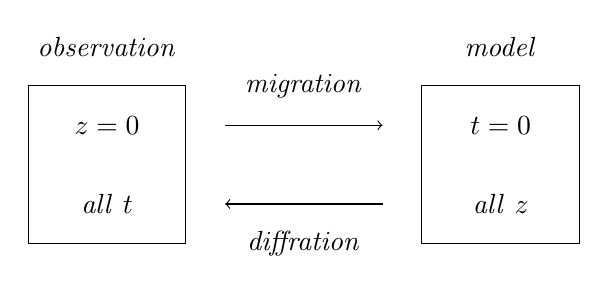
\begin{tikzpicture}
\centering
\draw (9,0) rectangle(11,2);
\draw (14,0) rectangle(16,2);
\draw[->] (11.5,1.5) -- (13.5,1.5);
\draw[<-] (11.5,0.5) -- (13.5,0.5);
\node at (10,0.5) {\emph{all} $t$};
\node at (10,1.5) {$z=0$};
\node at (15,0.5) {\emph{all} $z$};
\node at (15,1.5) {$t=0$};
\node at (10,2.5) {\emph{observation}};
\node at (15,2.5) {\emph{model}};
\node at (12.5,2) {\emph{migration}};
\node at (12.5,0) {\emph{diffration}};
\end{tikzpicture}

有时把绕射看作是形成与扩展双曲面的自然过程,偏移则是完成其反过程的计算机处理。


在第三章中将出现使用偏移一词的另一种情形,在该章中,水平坐标可以是炮点与检波点之间的中点$y$,
或者是炮检距$h$。在$(y,t)$平面和$(h,t)$平面内全都可以将双曲面向下
延拓,在$(y,t)$平面内,这种向下延拓称作偏移或成像,而在$(h,t)$平面内则将它称作聚焦或速度分析。


\subsection{数据资料中的脉冲}
惠更斯绕射在$(x,z)$空间内呈孤立的脉冲函数(即$\delta$函数)形式,从而$z=0$时在$(x,t)$
空间内就可使它成为一支双曲线。逆过程则需从$z=0$
时在$(x,t)$空间内的一个$\delta$函数开
始。这种倒过来的过程可以想像成是属于这样一类地震勘测:除了在一个特定位置上能记录
到回声之外,在任何其他位置上均记录不到,而在该特定位置上记录到的又仅只是一个回
声。同这样的观测结果符合一致的应该是什么样的地层模型呢?如图\ref{fig:xrf/semicirc}所示,这种地层
必须包含有一个球形反射面,球心就位于那个奇妙的记录位置上。
\begin{figure}[H]
\centering
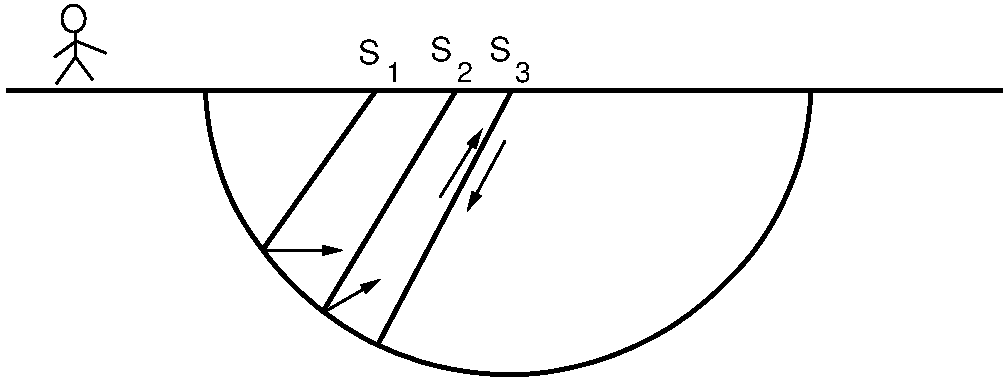
\includegraphics[width=0.6\textwidth]{xrf/semicirc}
\caption[semicirc]{当地震震源S准确位于半圆形反射面的圆心时,那时且仅仅在那时,才会有一个回声反射至
位于震源点上的检波器。这种半圆形反射面是根据仅只在地面一个位置上记录到一个回声这种数据记录方式作出的逻辑推论。}
\label{fig:xrf/semicirc}
\end{figure}

自然过程会在地层内部形成许多球形反射面,这看来是未必可能的。但是当我们注意业
经处理过的地球物理资料时,往往可看到剖面上有那么一些球形反射面。显然,这类输入数
据中包含有一些与此处所解释的波动传播理论不尽符合一致的脉冲。这点说明,为什么石油
勘探人员即使他们个人并不打算编写什么
处理程序,可他们却不得不研究反射地震数据处理方法。要理解认识原始数据资
料,那太复杂了。经过处理的资料可以给
出一个地层模型,但是它的可靠性难以断
定。你也许从未打算去造一辆汽车,但是
当你独自驾车远行进入沙漠时,那还是谨
慎一点好,应该尽你所能去了解熟悉关于
汽车的知识才是。

\subsection{手工偏移}

已知在点$(x_{0},t_{0})$上的地震同相轴 其斜率为$p=dt/dx$,试确定偏移后之位置$(x_{m},t_{m})$。
设想有一平面波阵面与地表面呈夹角$\theta$,在时间$dt$内传播距离为$dx$假设速
度为$v$,我们就得出以可观测量表示的波动传播角度

\begin{equation}
sin\theta=\frac{vdt}{dx}=pv
\label{eq:ex3}
\end{equation}

垂直旅行路程因
\begin{subequations}
\begin{equation}
t_{m}=t_{0}cos\theta=t_{0}\sqrt{1-p^{2}v^{2}}
\label{eq:ex4a}
\end{equation}

而小于有角度倾斜时的路程。由旅行时间$t_{0}$及速度水平分量$vsin\theta$得出偏移之后的横向位置为

\begin{equation}
x_{m}=x_{0}-t_{0}vsin\theta=x_{0}-t_{0}pv^{2}
\label{eq:ex4b}
\end{equation}
\end{subequations}

考虑到双曲线是向其顶点作偏移,就会明白为什么式\ref{eq:ex4b}中包含有一负号。式\ref{eq:ex4a}与
式\ref{eq:ex4b}是反射地震资料人工偏移的基本方程,它们告诉你偏移至何点,但是它们并未告
诉你斜率$p$会如何变化。

\subsection{反射面变陡}

设有一垂直分界面,这是倾斜地层的一种极限情形,它的反射,即双曲线的一支渐近线,却具有非垂直的陡实偏移将使倾斜地层的视陡度增大。
我采用视陡度一词,是因为
它是在$(x,t)$平面内所看到的已经变陡了的地层的斜率。偏移结果实际是沿$z$轴方向
分布的,但是为形成偏移时间剖面,总是使$z/v$重合在$t$轴上。当我们说一个双曲线偏移至其
顶点时,我们考虑的当然是偏移时间剖面。让我们将变陡过程作为一个角度函数来加以研究
一下。

设原点$(x_{0},t_{0})$邻近有一点$(x_{0^{+}},t_{0^{+}})=x_{0}+\Delta, t_{0}+p\Delta$,根据方程\ref{eq:ex4b},这个邻域偏移至

\begin{subequations}\label{eq:ex5}
\begin{equation}
t_{m^{+}}=(t_{0}+p\Delta)\sqrt{1-p^{2}v^{2}} \label{eq:ex5a}
\end{equation}
\begin{equation}
x_{m^{+}}=x_{0}+\Delta-(t_{0}+p\Delta)p^{2}v^{2} \label{eq:ex5b}
\end{equation}
\end{subequations}

现在我们可计算出偏移之后的同相轴因倾斜而形成的斜率$p_{m}$为

\begin{equation}
p_{m}
=\frac{dt_{m^{+}}}{dx_{m^{+}}}
=\frac{dt_{m^{+}}/d\Delta}{dx_{m^{+}}/d\Delta}
=\frac{p}{\sqrt{1-p^{2}v^{2}}}
=\frac{tan\theta}{v}
\label{eq:ex6}
\end{equation}

所以,像直角坐标空间内的斜率一样,偏移时间剖面上的斜率暗示着倾斜角度的正切,而未
偏移的时间剖面上的斜率则是该角度的正弦。

倾斜层在偏移时有斜率变化而双曲线的两翼在向下延拓时却未改变斜率,这事看起来
似乎有点自相矛盾,其实不然。一个原因是偏移等于向下延拓再加上成像(选择$t=0$时);
另一个原因则是一个双曲线是在一个深度上由一个震源所形成的一种特殊同相轴,而倾斜层
却是由不同深度的许多震源的叠加结果所形成。图\ref{fig:xrf/dip}即是表明形成一线状反射面
的许多点如何由绕射形成为一线形反射,以及形成一线形反射的许多点是如何偏移至一线状反射面的。

\begin{figure}[H]
\centering
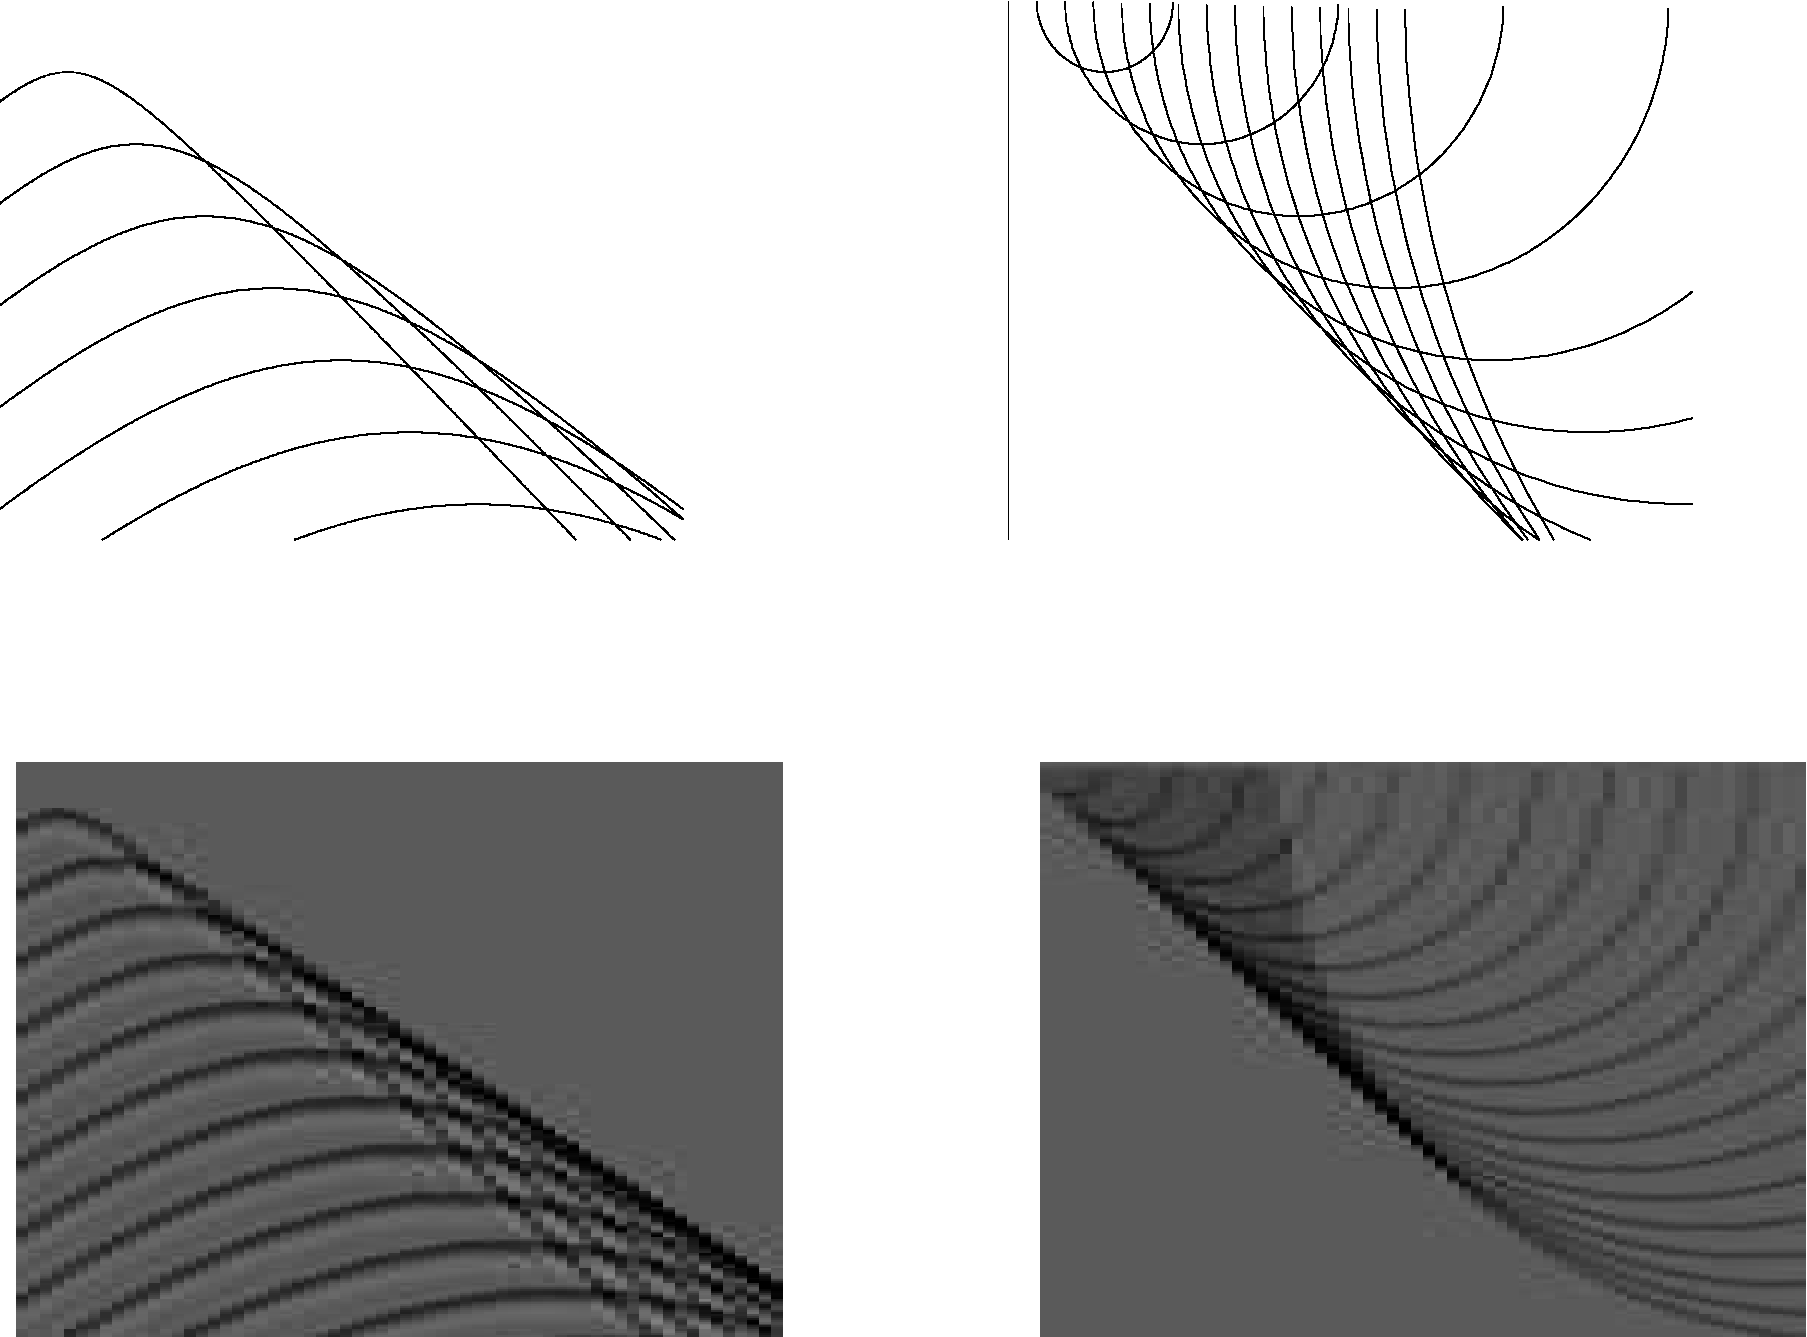
\includegraphics[width=0.95\textwidth]{xrf/dip}
\caption[dip]{
    左图是许多双曲线的叠加结果.各支双曲线顶部沿一条直线成布,该直线就像是反射面,不过并不是一条连
    续直线,而是一系列的点。相长干涉形成一个向一侧的视反射。
    右图表示许多半圆的叠加结果.各个半圆的底部沿一条直线分布,该直线代表观测到的平面波。不是平面波分
    解成一系列反射到达点,而是现在要把每个反射点解释成来自一个半圆状反射镜面。把所有反射镜面加起来,
    就形成了一个陡倾斜反射面。
}
\label{fig:xrf/dip}
\end{figure}
    
\subsection{爆炸反射面概念的限制}
    爆炸反射面概念是有力而又巧合的类比
    对于全部时间是从事于解释而不是从靡于处理
    的人来说,将爆炸反射面概念喻之为必不可少的拐棍还不够,它还是仅有的运输工具!可是
    对于我们这些从事于数据处理的人来说,这个爆炸反射面概念却有一个严重的缺点,现在还
    没有一个人已经解决了如何把这概念推广应用于非零炮检距记录资料的问题,
    资料却都是以相当大的炮检距进行记录的。在现代海上地震勘探中,不是用
    而是成百个串接在一条电缆上,拖在船后。记录系统的电缆长度典型的是二至三公里,勘探
    钻井可达三公里左右的深度,所以,实际上,地层倾角可以很大.这就涉及到新问题和新机
    会了,不过所有这些要到第三章才会讨论。
    
    再者,即使是零炮检距记录,这个爆炸反射面概念在定量上也不正确.该概念能有效成
    立的范围,将在第三章中阐述,此刻只对三个明显缺点作些注释:图\ref{fig:xrf/fail}所示是无法用爆
炸反射面模型加以预测的射线,这类射线在零炮检距剖面中却会出现。为适应这种情况,就
    只得假设存在有速度横向变化。

\begin{figure}[H]
\centering
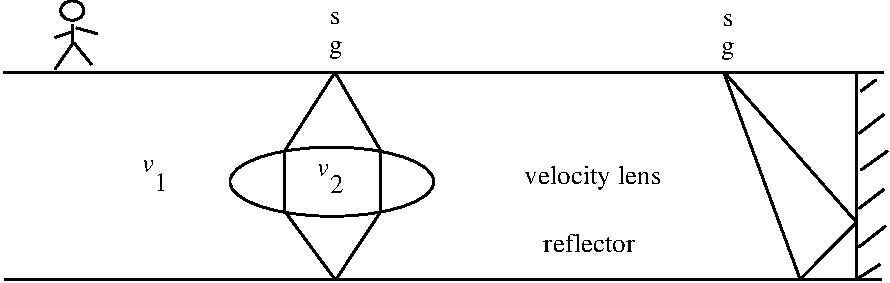
\includegraphics[width=0.95\textwidth]{xrf/fail}
\caption[fail]{
爆炸反射面模型解释不了的两支射线,然而零炮检距剖面上却可能存在这种射线。
}
\label{fig:xrf/fail}
\end{figure}
其次,爆炸反射面概念无法解释多次反射。设有双程波旅行时间为$t_{1}$的一个平缓海底,由
海底形成的多次反射应在时间$2t_{1},3t_{1},4t_{1}...$等可预测到,而按照该爆炸反射面概念
来解释,则第一次的多次反射应该从反射面至海面然后由海面至反射面,再从反射面至海面,总时间为
$3t_{1}$,从而相继的多次反射应在时间$5t_{1},7t_{1}...$
时出现。由此可知,零炮检距剖面上产生的多次反射不同于爆炸反射面模型产生的那些多次
反射。
    
我们能够看到波从分界面的两侧发生反射,这就涉及到爆炸反射面模型的第三个缺点,   
爆炸反射面模型预言由两侧出射的波具有相同极性,而根据反射系数的物理意义则只能说相
反两侧所形成的反射应具有相反极性。    
\subsection*{板块构造例子}
  板块构造理论认为,洋底是由海洋中部附近的脊火山上所形成的薄板块构成的,这些板
  块向海洋最深部的海糟移动,在那里它们倾没重返地壳。对该理论最有利的证据就是洋底缺
  失古老的岩石,一般而言,大陆都是被较年轻的移动海洋板块所推挤碰撞的古老岩石。有很
  多种方法可以极容易地观察到洋中脊火山作用形成的板块建造,至于板块是否真正在海槽中
  碰撞那就无法观测如此清晰了.证据均来自天然震源位置和反射地震学,图\ref{fig:xrf/japan}所示是
  日本海槽的一些反射资料,有两组反射占优势地位,即海底反射和向左方下倾的较深地层,
  后者可假设是开始倾没入地壳的一个板块的顶部;像近地面张力断裂那样,我们可将它作为
  向下挠曲的证据来加以研究(最顶部地层是与板块作松散接触的新近沉积海相软地层)。
  
\begin{figure}[H]
\centering
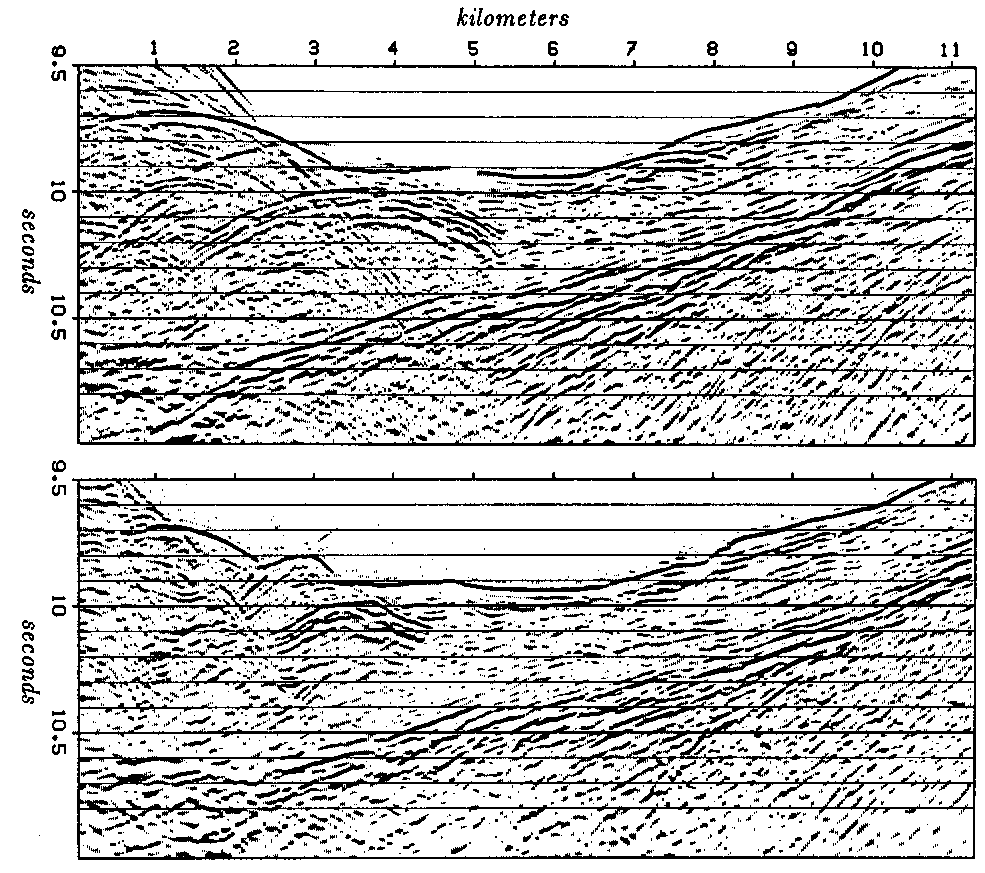
\includegraphics[width=0.95\textwidth]{xrf/japan}
\caption[japan]{
    上图是通过日本海槽的一条11公里长的测线的反射资料(东京大学海洋学研究所),下图所示为
    偏移处理之后的结果(Ottolini)
  }
\label{fig:xrf/japan}
\end{figure}
  注意,图\ref{fig:xrf/japan}的顶部不是零时间,时间轴是从9.5秒至11.0秒,在9.5秒以前没有反射
——我们要等待波在船与洋底之间传播。1公里至3公里周围的双曲线形反射同相轴因偏移归位形成为引人兴趣的``块状''。注意看一下8公里附近的海底地形和偏移与未偏移剖面之间的
  差异。偏移之后,的绕射双曲线就从4公里处的板块反射附近消失了,许多断裂(尤其
  是6.2公里处的一个断裂)都能更为明确地解释了。最后,如板块是向下挠曲,可是根据所
给资料,这点并不明显,要解决这个有关挠曲的疑问实际上还得要求对地震速度的横向变作更详尽的分析。

作为一个具体石油勘探意义的例子,看一下图\ref{fig:xrf/growth},这是德克萨斯州海上勘探的资
料,沉积物在沿岸河流进入墨西哥海湾处沉降,增加的重量引起沿着陡断层发生滑塌。在钻
井可以证实有一透水砂岩层之后,可将相应之反射沿上倾方向外推,与图\ref{fig:xrf/growth}资料上那
  样一些最邻近的断层倾斜相接.该断层很可能破坏了形成烃类向上运移聚集的渗透性通道的
  连续性。在这个深度上的砂岩可具有25热的孔隙率。假定地震波速度为2.2公里/秒,从而可
  导出图\ref{fig:xrf/growth}资料与实际物理体积之间的比例关系,对含油体积与图\ref{fig:xrf/growth}上同一体积的比
  值进行比较,可作出储量判断,由此你就可明白良好的成像是有多么重要了。

\begin{figure}[H]
\centering
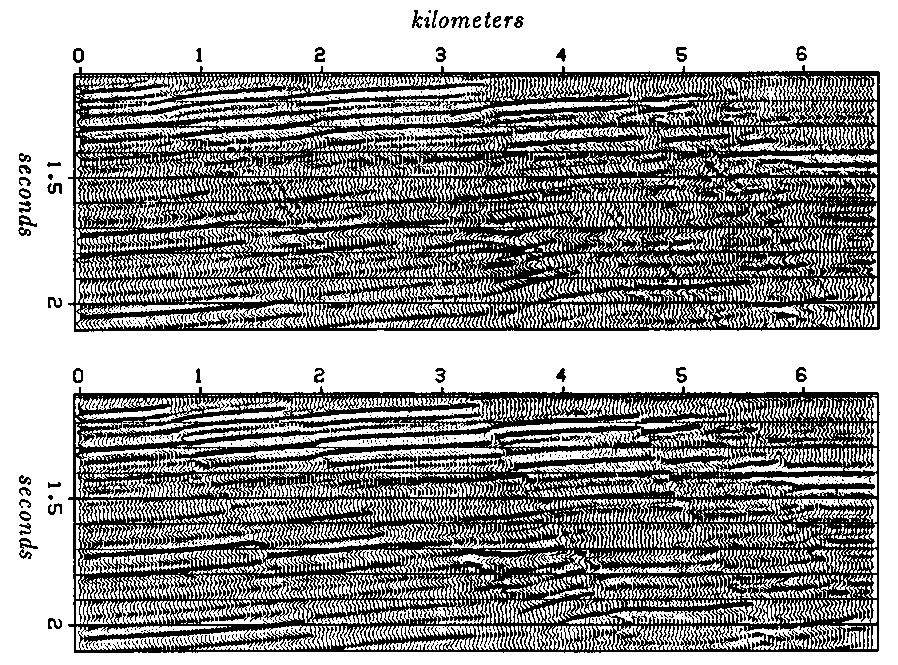
\includegraphics[width=0.95\textwidth]{xrf/growth}
\caption[growth]{
    上图是墨西哥海湾沿得克萨斯海岸海上勘探测线的6.5公里长的反射资料;下图为
      偏移处理的结果(Rothman )
  }
  \label{fig:xrf/growth}
\end{figure}

\subsection{习 题}

\begin{enumerate}
\item
    试证明毕达哥拉斯定理,即:直角三角形的斜边长度付决定于关系式$x^{2}+z^{2}=v^{2}t^{2}$。
\item 
    试计算图\ref{fig:xrf/japan}中双曲线两翼的传播角度
\item

利用习题2所得结果导出板块的倾伏角度。
\item 
试问日本海槽有多深(水层速度为1.5公里/秒)?
\item 
    试问在图\ref{fig:xrf/growth}上外海位于何方向?为什么?
\end{enumerate}

\begin{figure}[H]
\centering
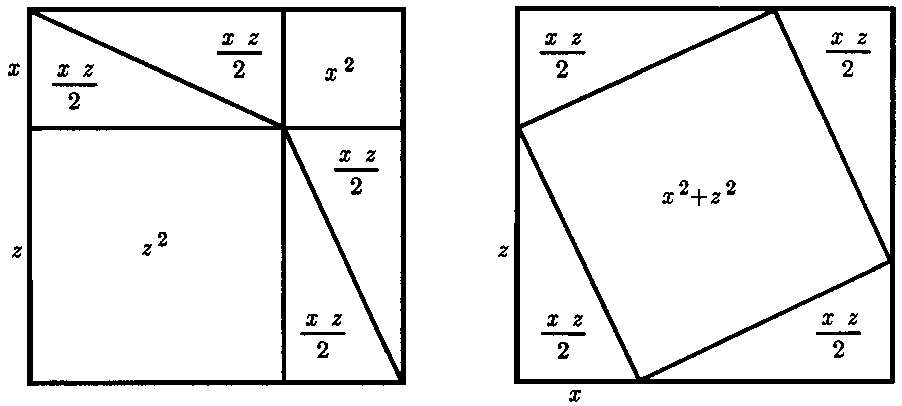
\includegraphics[width=0.95\textwidth]{xrf/pythag}
\caption*{
  
}
\label{fig:xrf/pythag}
\end{figure}

